%%%%%%%% ICML 2015 EXAMPLE LATEX SUBMISSION FILE %%%%%%%%%%%%%%%%%
%%%%%%%%%%%%%%%%%%%%%%%%%%%%%%%%%%%%%%%%%%%%%%%%%%%%%%%%%%%%%%%%%%

\documentclass{article}

\usepackage{times}
\usepackage{graphicx}
\usepackage{subfigure} 

% For citations
\usepackage{natbib}

% For algorithms
%\usepackage{algorithm}
%\usepackage{algorithmic}
% Packages hyperref and algorithmic misbehave sometimes.  We can fix
% this with the following command.
%\newcommand{\theHalgorithm}{\arabic{algorithm}}

\usepackage{hyperref}
\usepackage{amsmath}
\usepackage{amssymb}

\def \N {\mathbb{N}}
\def \Nbr {\mathcal{N}}
\def \Q {\mathbb{Q}}
\def \F {\mathbb{F}}
\def \then {\implies &}
\def \oif {\Longleftrightarrow &\,}
\def \given {\text{Given }&}
\def \assume {\text{Assume }&}
\def \thfr {\therefore &\enskip}
\def \bij {\leftrightarrow}
\def \inj {\rightarrowtail}
\def \sur {\twoheadedrightarrow}
\def \R {\mathbb{R}}
\def \C {\mathbb{C}}
\def \D {\mathbb{D}}
\def \iff {\Longleftrightarrow}
\def \kron {\boldsymbol\delta}
\def \id {\text{id}}

\def\Tx{\textbf{x}}
\def\Ty{\textbf{y}}
\def\quotient{\mathclose{}/\mathopen{}}
\def\Tf{\textbf{f}}
\def\Th{\textbf{h}}
\def\Tg{\textbf{g}}
\def\sumn{\sum_{n=0}^\infty}
\def\limn{\lim_{n\rightarrow\infty}}
\def\prodn{\prod_{n=0}^\infty}
\DeclareMathOperator\adj{adj}

\newcommand{\stc}[1]{\widetilde{#1}}   
\newcommand{\pa}[1]{ \left({#1}\right) }
\newcommand{\set}[2]{ \left\{ #1 \,\middle|\, #2 \right\} }
\newcommand{\shift}[1]{&\quad & \text{#1}\\}
\newcommand{\lem}[1]{\text{\textbf{L.\ref{#1}}}}
\newcommand{\card}[1]{\left\vert{#1}\right\vert}
\newcommand{\Ps}[1]{\mathcal{P}\left({ #1 }\right)}
\newcommand{\colv}[1]{\begin{pmatrix} #1 \end{pmatrix}}
\newcommand{\mat}[1]{\begin{pmatrix} #1 \end{pmatrix}}
\newcommand{\detmat}[1]{\begin{vmatrix} #1 \end{vmatrix}}
\newcommand{\spanb}[1]{\text{span}\{ #1 \}}
\newcommand{\abs}[1]{\left|#1\right|}
\newcommand{\Inner}[1]{\langle #1 \rangle}
\newcommand{\Innercpy}[1]{\langle #1, #1 \rangle}
\newcommand{\conj}[1]{{\overline{#1}}}

\DeclareMathOperator{\Tr}{tr}
\DeclareMathOperator{\Dim}{dim}
\DeclareMathOperator{\Rank}{rank}
\DeclareMathOperator{\Ker}{ker}
\DeclareMathOperator{\Diam}{diam}
\DeclareMathOperator{\Diag}{diag}
\DeclareMathOperator{\Int}{int}
\DeclareMathOperator{\Clo}{clo}
\DeclareMathOperator{\sgn}{sgn}
\DeclareMathOperator{\MyRe}{Re}
\DeclareMathOperator{\MyIm}{Im}
\DeclareMathOperator{\res}{res}

% Employ the following version of the ``usepackage'' statement for
% submitting the draft version of the paper for review.  This will set
% the note in the first column to ``Under review.  Do not distribute.''
%\usepackage{icml2015} 

% Employ this version of the ``usepackage'' statement after the paper has
% been accepted, when creating the final version.  This will set the
% note in the first column to ``Proceedings of the...''
\usepackage{icml2015}


% The \icmltitle you define below is probably too long as a header.
% Therefore, a short form for the running title is supplied here:
\icmltitlerunning{Commodities Forecasting with GDELT}

\begin{document}
\twocolumn[
\icmltitle{Commodities Forecasting from Non-Financial World News from GDELT}

% It is OKAY to include author information, even for blind
% submissions: the style file will automatically remove it for you
% unless you've provided the [accepted] option to the icml2015
% package.
\icmlauthor{Vladimir Feinberg}{vyf@princeton.edu}
\icmladdress{Princeton University}
\icmlauthor{Ghassen Jerfel}{gjerfel@princeton.edu}
\icmladdress{Princeton University}
\icmlauthor{Daway Chou-Ren}{dchouren@princeton.edu}
\icmladdress{Princeton University}
\icmlauthor{Zi Xiang Pan}{zpan@princeton.edu}
\icmladdress{Princeton University}
\icmlauthor{Tom Wu}{tongbinw@princeton.edu}
\icmladdress{Princeton University}

% You may provide any keywords that you 
% find helpful for describing your paper; these are used to populate 
% the "keywords" metadata in the PDF but will not be shown in the document
\icmlkeywords{GDELT, commodities, finance, forecasting, clustering, machine learning, ICML}

\vskip 0.3in
]

\begin{abstract} 

We propose a new method for predicting commodity price data through the use of aggregated daily non-macroeconomic news. Our method creates a static clustering to extract topics and weights each day's news events with an extracted importance metric. We use the GDELT news database to extract raw news attributes and sentiment evaluations of the articles. With a $K$-means model for clustering news data feeding into an a lasso regression model as a prediction for the log returns on commodity price will for the next day, [TODO(Ghassen) l1 model accuracy]. When using a Kelly criterion based trading strategy, we gained [TODO(Vlad) returns] when training on ? days and testing on ? [TODO(Vlad)].
\end{abstract} 

%TODO review below
% Submissions must be in PDF.
% The maximum paper length is \textbf{8 pages excluding references, and 10 pages including references} (pages 9 and 10 must contain only references).
% Do \textbf{not include author information or acknowledgments} in your initial submission. 
% Your paper should be in \textbf{10 point Times font}.
% Make sure your PDF file only uses Type-1 fonts.
% Place figure captions {\em under} the figure (and omit titles from inside the graphic file itself).  Place table captions {\em over} the table.
% References must include page numbers whenever possible and be as complete as possible.  Place multiple citations in chronological order.  
% Do not alter the style template; in particular, do not compress the paper format by reducing the vertical spaces.

\section{Introduction}

TODO(Daway): Sections 1 - 3: cut down and incorporate edits from midterm grades (and relevant parts of section 4)

TODO(Vlad): Trading strategy
 
Financial data prediction is appealing both for its challenging nature and for its practical applications. Because market dynamics are complex and random, accurate price prediction is difficult. There are two types of market prediction techniques: fundamental analysis, which relies on an asset's data for forecasting, and technical analysis, which relies on historical trends to exploit market timing \cite{schumaker2009textual}. This paper examines the use of news data to augment technical analysis for prediction of commodity prices. We assume there is a set of news basis vectors that is stable over time which can be used for this purpose. %TODO: keep last sentence?

We focus on a comprehensive set of non-economic news data unrelated to financial markets, interest rates, stock prices, and the like. In particular, we will analyze whether a summary of a day's news topics is predictive of commodity prices the next day. To avoid losing information about the significance of singular events, we will rely on the sentiment analysis already applied to our dataset to calculate how each news event should be weighted in a daily news summary.

\subsection{Commodity Prediction}
We choose to predict commodities prices because while various studies have analyzed the effect of news on stock prices \cite{mcqueen1993stock} and foreign exchange rates \cite{kamruzzaman2003svm}, relatively little work has looked at applying news data to the prediction of the similar commodities market. The use non-economic news because the influence of economic news has already been examined in the past by many researchers \cite{gidofalvi2001using}\cite{schumaker2009textual}\cite{bollen2011twitter}\cite{hagenau2012automated}. We believe real-time news information has predictive power for commodity prices, because, since commodities, by definition, must be extracted or produced by countries, it is likely that underlying factors of their production rates will be captured by local news, especially reporting on crisis events. Prices are also sensitive to current conditions because the supply and demands that drive them are inelastic, or unaffected by changes in price \cite{chen2008can}. 

\subsection{GDELT Dataset}
We draw news from the Global Database of Events, Language, and Tone \cite{GDELT}, which aggregates news from broadcast, print, and web sources across 100 languages and parses out features to describe each news event. Each news event has 58 features which can be broadly divided into either topical or importance-related data. Topical data might include the two actors involved in an event, the general sentiment of the language used, the location of actors, or broad categorization of the type of event occurring (trade agreement, violent action, etc) in categorical codes (CAMEO codes). Importance-related features deal with the magnitude of the event and are drawn from metrics such as the number of news sources mentioning the event, or the total number of articles written about it. GDELT is available for free and uses a variety of international news sources with daily updates, and contains more than 250 million events from 1979 to present, or roughly 100,000 per day. GDELT's predictive potential for financial markets has been positively assessed by researchers who used GDELT to examine the impacts of the June 2013 Southeast Asian heat wave and the December 2013 Indian riots and the effect they had on the Singapore stock market \cite{phua2014visual}.

 
\section{Motivating Analysis}


\subsection{GDELT Dataset}

\subsubsection{Sparsity in GDELT}

The space of news events spanned by all columns in GDELT is much larger than the subspace we expect news to lie on. Confirming these suspicions is important because it would indicate a need to reduce the dimensionality of the data set we are working with.

Classical dimensionality reduction was not tractable to apply to a dataset of this size - the highly categorical nature of the dataset results in a large dimensional expansion when preparing numeric inputs to the algorithms. A fast neighborhood-embedding method, tSNE, relies only on a metric between data points. Unfortunately, its runtime and space consumption grows exponentially in the reduced dimension, and extremely small dimensions yielded poor results \yrcite{van2008visualizing}.

However, it is critical to observe some sparsity in the GDELT space to confirm our clustering-based approach.

We guessed that there are likely to be at least two modes of low-dimensional interactions in the data: (1) that actors only interact within small cliques and (2) that each actors to small sets of events. We conducted this initial analysis on a random sample of days before August 2015 to avoid making conclusions that overfit the test data.

\begin{figure}[ht]
\vskip 0.2in
\begin{center}
%\centerline{\includegraphics[width=\columnwidth]{}}
\caption{
BOX WHISKER HERE. DESCRIBE 5 FIGURE SUMMARIES, OUTLIER
}
\end{center}
\vskip -0.2in
\label{fig:events-per-actor}
\end{figure} 


\begin{figure}[ht]
\vskip 0.2in
\begin{center}
%\centerline{\includegraphics[width=\columnwidth]{}}
\caption{TODO: take another random sample, histogram it. Describe summary stats. number of Distinct events per actor.}
\end{center}
\vskip -0.2in
\label{fig:events-per-actor}
\end{figure} 


As Figure \ref{fig:actors-per-actor} demonstrates, actor count is heavily skewed distribution. This gives us confidence in (1) for the sampled days. We conduct a similar inspection for the number of unique CAMEO coded events per actor in Figure \ref{fig:events-per-actor}:

\begin{figure}[ht]
\vskip 0.2in
\begin{center}
%\centerline{\includegraphics[width=\columnwidth]{}}
\caption{TODO: take another random sample, histogram it. Describe summary stats. number of Distinct events per actor.}
\end{center}
\vskip -0.2in
\label{fig:events-per-actor}
\end{figure} 

In addition to more compact data representation and reduction of noise, dimensionality reduction has several other attractive features for this dataset. First, it enables us to work in a continuous space of reduced-dimension tuples of real values, which is much easier for model generation than partially categorical variables. Secondly, the large volume of the data set implies that any size reductions that can be gained will result in more manageable data pipelines

\subsection{Bloomberg Commodity Prices}

up and down spikes

normally distributed about 0

\section{Related Work}

On the whole, predicting any financial market has proven to be difficult. Simon's work encapsulates many of the inherent problems. Model evaluation cannot rely on using normal RMSE metrics, which might suffer from lag problems, but must either demonstate ability to generate profit through a trading scheme or demonstrate an ability to correctly predict directionality for desired trading period times. Simon identifies a training period of 3 years and a test period of 6 months as optimal \cite{forex_neuralnets}.

\noindent In an examination of the potential for technical approaches to predict pricing movements, Gidofalvi found that a 20 minute period before and after the release of financial news allowed for a weak prediction of price movements \cite{gidofalvi2001using}. It was found by McQueen and Roley that fundamental macroeconomic news has little impact on stock prices but that other news types have effects dependent on responses of expected flows relative to equity discount rates \cite{mcqueen1993stock}.\\

\noindent In addition to Phua et al's work in identifying crisis points in Singapore's stock market, Schumaker and Chen were able to demonstrate 57\% directional accuracy when using news articles to predict S\&P500 stocks in Gidofalvi's 20 minute period \cite{schumaker2009textual}. Bollen et al also achieved an accuracy of 86.7\% when incorporating semantic mood data from Twitter \cite{bollen2011twitter}. Other research has focused on extracting semantics from blogs or financial news. Hagenau et al show that context-specific feature extraction from news can reduce overfitting of models \cite{hagenau2012automated}.\\

\noindent The work done by Phua et al is important for validating GDELT in particular as a valid news source for market prediction. Topic analysis shows that GDELT includes impactful events across multiple iterations of clustering (thus correctly assigning impactful events large magnitudes) and also correctly chronologically tracks changing magnitudes. Term extraction from news sources is shown to be relevant using concept link exploration. Phua et all do find that not all significant events can be discovered by GDELT. They were also unable to verify that quality for semantic score assignments was high.

\section{Methods}


Recent GDELT updates provide feeds with 15-minute resolution \cite{GDELT2}, but historical feeds offered only daily resolution. We decided for simplicity to analyze daily changes in price, taking a full day's worth of news data into account. This was most in line with testing our hypothesis, that an aggregation of topic clusters in a day's news is predictive of commodity pricing.

Our data pipeline was designed to provide day-wise parallelism over our data set in order to enable fast testing of new feature extraction methods. The raw data, as well as intermediate data, is stored in TSV ASCII format.

\subsection{Model}

Every news event in GDELT is stored as a row in a file for that day's report. Every set of rows may undergo a series of transformations. First, in the \textbf{preprocessing} stage, we extract relevant topic- and importance- related columns. For topics, a mix of numeric and categorical fields are extracted. Importance columns are saved for use in a further step. Next, in the \textbf{expansion} stage, we project each row of topic features to a purely real space by using one-hot encoding for categorical values. For each category, one-hot encoding produces $n$ dummy boolean variables, where $n$ is the number of unique categories. Finally, in the \textbf{summary} stage, $K$-means clustering is performed on this purely numeric representation of the data. Euclidean distance is used as the distance metric for $K$-means. Many clustering models are created with a range of $K$ from 10 to 5000.

The day summaries are then conglomerated in a time series $\{\textbf{d}_i\}$. For a day-indexed time series of a commodity's price, $\{p_i\}$, we have the corresponding sequence of binary labels indicating whether price has increased the next day, $y_i=1_{p_{i+1}>p_i}$.

Thus, our model assumes that:
\begin{enumerate}
\item The static clustering of news topics is accurate for the future.
\item $\mathbb{P}(p_{i+1}>p_i)$ may be determined by a regression over summaries $\textbf{d}_i$. 
\end{enumerate}

Both of these are strong assumptions. The first may be weakened by adapting a dynamic clustering model, such as an infinite Gaussian Mixture Model or a Hierarchical Dirichlet Process. The second requires $\textbf{d}_i$ to be both contain a sufficient amount of information to predict price behavior, which is a matter of appropriate feature extraction, and the assumption that we do not lose too much predictive power in summarizing a day by aggregating over the clusters to which its news events belonged.

\subsection{Execution}

Our current implementation uses $K$-means for clustering and logistic regression for classification. We trained, validated, and sampled from the days between 2006-01-01 and 2015-07-31. Recent days were used for testing.

For tractability reasons, we use a random sample of one million events to create the clustering models which are used in the main pipeline. This sample goes through the same preprocessing and expansion pipeline as the day summaries which are used in the regression except its output is used to create a clustering model. The sample is drawn uniformly from all events without any recency bias.

The raw data starts with $X=58$ columns. Each day has around $N=100,000$ rows. The total size of the set is about 60GB. %TODO precise mean and stddev.

\begin{figure}[ht]
\vskip 0.2in
\begin{center}
\centerline{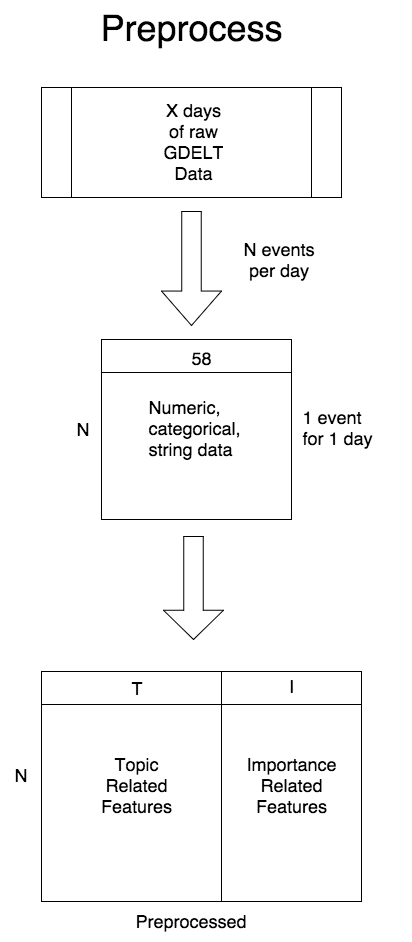
\includegraphics[scale=0.15]{images/preprocess_vertical.png}}
\caption{Preprocessing stage}
\end{center}
\vskip -0.2in
\label{fig:preprocess}
\end{figure}

The preprocessing step does standard data cleaning, removes all but 19 of the original columns, and also groups them into $T=12$ topic-related columns and $I=9$ importance columns. The topic columns are in a compressed format, with categorical variables represented as integers. String columns are sanitized and have stop words removed.

\begin{figure}[ht]
\vskip 0.2in
\begin{center}
\centerline{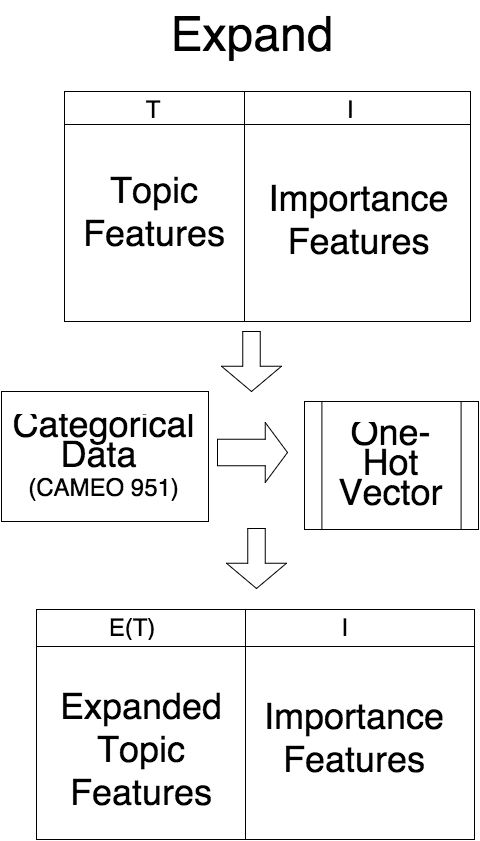
\includegraphics[scale=0.15]{images/expand_vertical.png}}
\caption{Expansion stage}
\end{center}
\vskip -0.2in
\label{fig:exapand}
\end{figure}

The expansion step one-hot encodes categorical features, such as the event CAMEO codes,  producing $n$ dummy boolean variables, where $n$ is the number of unique categories.

%TODO mention here that we do sample-mean and sample-std-dev-based scaling, once we actually do that

\begin{figure}[ht]
\vskip 0.2in
\begin{center}
\centerline{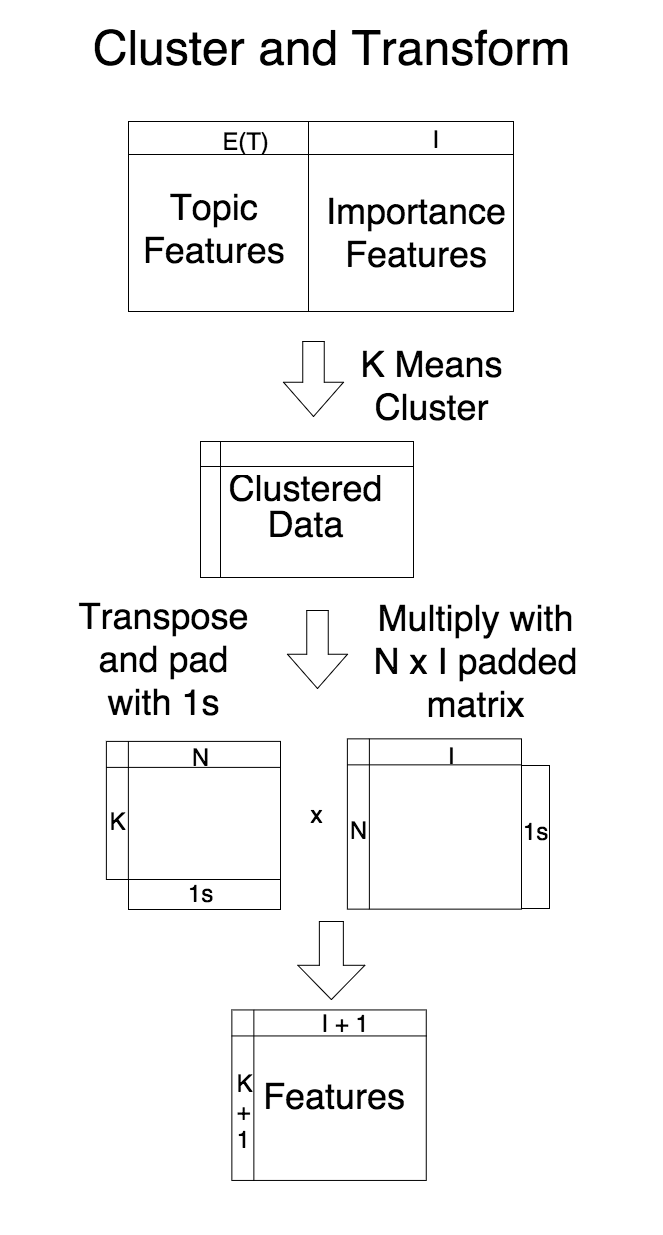
\includegraphics[scale=0.15]{images/cluster_and_transform_vertical.png}}
\caption{Summary stage}
\end{center}
\vskip -0.2in
\label{fig:summarization}
\end{figure}

Because of the padded $1$s in the $K+1$x$N$ and $N$x$I+1$ matrices from \ref{summarization}, their multiplication conveniently extracts the sum of importance-weighted events belonging to certain topics. Note that this model is extensible to a mixture model, where each event's contribution to a topic's importance for that day is weighed by the probability of belonging to that topic's class. Furthermore, the aggregation creates a uniform description of every day, a flattened vector of dimension dependent on the cluster count.

These daily summaries are then enriched with historical pricing data before being fed into the linear model. The pricing data added are the 5, 10, and 30 day rolling averages of the commodity price. %TODO hyperparam selection of rolling mean.


\subsubsection{Autoregressive Models: ARMA}
%TODO ghassen add a transitioning sentence
We started our exploratory analysis with binary classification. We used diverse classification techniques such as Linear Regression and SVM on the sign of the change of the returns from a day to the next. However, our accuracy results were sub-par. Therefore, we decided to employ Autoregressive models which combine the news data with the time series data in order to produce continuous predictions of next-day time series values. %%TODO: TOM
Autoregressive models are some of the most flexible and easy to use models for time series. The future value of a variable, in an AR model, is assumed to be a linear function of several past observations and random errors. Accordingly, AR models have proven to be especially useful for describing the dynamic behavior of economic and financial time series and for forecasting \cite{tsay, VAR}. Recent literature proved their superiority in financial modeling to most other techniques such as Neural Nets and SVM. %%TODO: G reference
\\
The basic p-lag vector autoregressive model (AR(p)) has the form: $$\bf{Y}_t=\bf{c}+\bf{\Pi}_1\bf{Y}_{t-1}+\bf{\Pi}_2\bf{Y}_{t-2}+\cdots+\bf{\Pi}_p\bf{Y}_{t-p}+\epsilon_t,$$ $$t=1\ldots T$$ with $\Pi_i$ being the coefficients and $\epsilon_t$ is an unobservable zero mean noise. We can also do subset-autoregression where we pick multiple specific lags instead of a full range of lags like the basic AR(p) would do as show in the previous equation.
One of the most common extensions to Autoregressive models is to include moving averages and integration terms that take into account the stationarity of the time series. This is what constitutes Auto-Regressive Integrated Moving Average (ARIMA) models. They are  the most general class of models for forecasting a time series which can be made to be “stationary” by differencing (if necessary), perhaps in conjunction with nonlinear transformations.
Accordingly, an ARIMA model is fully determined by 3 parameters, one for each of the (AR),(I) and (MA) components: %%TODO: formatting
* p = order of autocorrelation for (AR)
* d = order of integration (differencing) for (I)
* q = order of moving averages for (MA)
Determining these orders can be done either visually using the Autocorrelation Function plot (finds the autocorrelation coefficients mentioned earlier) and the Partial Autocorrelation Function plot (correlation conditioned on other lags' autocorrelation) [Figure \ref{fig:ACF}] or analytically using a goodness of fit measure (which order fits the data best).
ACF or PACF plots indicates which lags are most correlated within the time series. They can be used to gauge if there is any sort of autocorrelation within the time series. They can be also be used to determine the exact orders depending on how the values in the plots decay or simply cut off but we're not covering those methods as we focused on the more methodical analytical approach.
\begin{figure}[ht]
	\vskip 0.2in
	\begin{center}
		\centerline{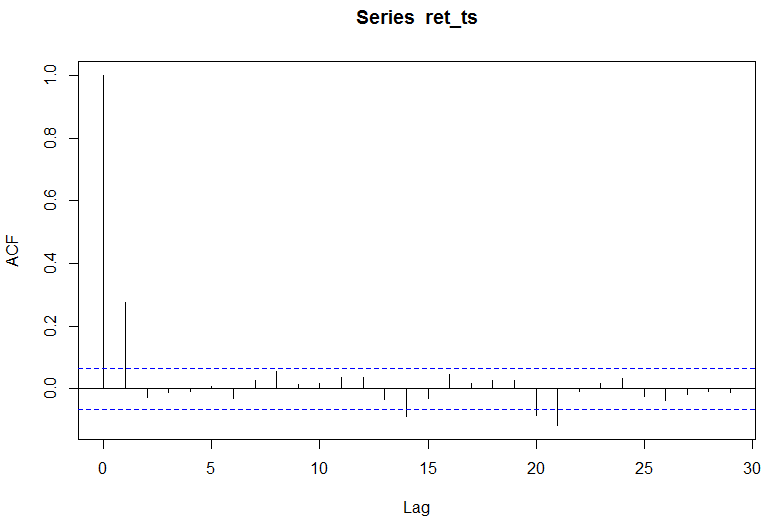
\includegraphics[width=\columnwidth]{ACF.png}}
		\caption{Autocorrelation Function plot for gold. Lags exceeding the dotted blue line have a statistically significant correlation with the 0-lag.Accordingly, the lags at 1, 14, 20 and 21 are correlated with the 0-lag (current time series).}
	\end{center}
	\vskip -0.2in
	\label{fig:ACF}
\end{figure}
For the goodness of fit, we had the options to use the Akaike information criterion (AIC), the Bayesian information criterion (BIC) or several other criterions that are more or less similar. These criterions would allow us to comapare the goodness of fit of different models, indexed by their parameters. Accordingly, we would be able to decide the best order or parameters for our model based on the set that achieves the best fit. Later, we will discuss which subset of the data this fit was tested on.
%%TODO G: Add the equations for AIC/BIC
For this paper, We decided to use the AIC which aims to choose a model that minimizes the KL divergence between the true density and the density of the MLE of a fixed model. Accordingly, the best model is the one with the lowest AIC. However, AIC is prone to overfitting and chooses predictive models over parsimonious ones. Given the literature's emphasis on the lack of predictive power in the domain of financial prediction, we decided to favor the predictive capacity over sparseness, for the order estimation, at least. BIC, on the other hand, favors sparsity over the predictive capabilities.
However, before testing the goodness of fit of different combinations of p and q parameters, we can figure out the d parameter using an Augmented Dickey Fuller test to verify the non-stationarity hypothesis of our data. Notice that random variable is stationary if its statistical properties are constant over time. Accordingly, it would have no trends and all of the variations around its mean would be random noise of constant amplitude. \cite{tsay, VAR}
If our data is already stationary, then there is no need for differencing (determining by the d component). In our case, for example, the non-stationary hypothesis was rejected with a p-value of 0.01 in the ADF test. Therefore, the d parameter that best fits our data is 0.
\subsubsection{Possible Extensions and Optimizations}
One possible extension to ARIMA or any time series model, for that matter, is adding a Markov Switching Model that assumes the existence of latent regimes and builds an independent model for each regime because.\cite{MS} After testing, we couldn't find any significant regimes in our training data which might infer that our regimes are over longer periods of time than that spanned by our data.
A possible optimization, which we benefited from, is the use of simple linear models (or generalized linear models) to simulate the AR component of ARIMA in case the (MA) component was deemed superfluous. In this case, we can build a simple design matrix where each column is a lagged version of the response variable. This design matrix can be used for a standard Ordinary Least Squares regressions as well as various other models that are computationally faster than ARIMA (with respect to their R implementations, at least).
\subsubsection{News Data: Exogenous Factors}
Our news data that we extract from GDELT is considered an exogenous factor. In the time series literature, there have been several approaches to including such information into time series models. The most two prominent methods are impulse responses or simply considering the exogenous data as time series to be evaluated alongside the financial times series (the way you'd do in a regression) such as in ARIMAX models (ARIMA + Exogenous).
The impulse response method attempts to detect impulses, whose response or effect decays with time,  within the time series data in order to localize the date of origin. Consequently, one would try to match the dates of such impulses with our news data in order to detect which columns in our data are most correlated with the big changes in those dates.
ARIMAX is simpler and more efficient, in literature and from our experience, especially with our linear models simplification. We add the columns of the news as extra time series whose autocorrelation with the response variable is evaluated in training. Note however that we use a lagged version of the news since our hypothesis is that the news from day D would affect the market after day D's closing which will be reflected on the difference of the values between D+1 and D.
\subsubsection{Column Selection of News Data}
However, a large number of columns in the news data (800 in the case of 100 clusters of GDELT data) can easily cause overfitting since the large number of variables could fit arbitrary data points to the noisy news columns. Accordingly, our out-of-sample testing results would suffer.
Another problem with a large number of columns is that ARIMA (the original implementation) and Ordinary Least Squares regression require the number of features to be less than or equal to the number of observations. This can be limiting as we would like to test different numbers of trainign days. Therefore, we recurred to Principal Component Analysis (among other methods that we tried) to reduce the dimensions. PCA converts a set of observations of possibly correlated variables into a set of values of linearly uncorrelated variables called principal components.\cite{PCA} One can select a fixed number of principal components that express most of the variance in a certain data set. In our case, we selected a number of principal components that accounted for $99\%$ of the variance in our data and used those principal components of the news data for the training as exogenous factors, instead of the original news columns.
\subsubsection{L1-regularizatio: Lasso Regression}
We also tried L1-regularization with Lasso regression since it inherently handles overfitting by enforcing sparsity, as compared to pre-emptively regularizing based on the variance, as in the case of PCA. \cite{glmnet} Lasso's sparsity is based on the actual importance of each column to the response variable and allows us to select a small number of explanatory variables. Additionally, Lasso doesn't require the number of variables to be less than the observations which allows us to test a small number of observations without applying any dimension reduction beforehand.
%%TODO GHASSEN: Explain Lasso More
Additionally, Lasso is computationally efficient as compared to other sparse regressions.\cite{glmnet} Finally, we can select the degree of our sparsity by selecting a Lambda coefficient which helps us better gauge the change of the predictive power of our model.
Accordingly, we build Lasso model with the minimum Lambda as defined by cross-validation and then use that model to estimate our log-returns for each training window.
\subsubsection{Testing Measures}
For out-of-sample testing, we used two measures to evaluate the prdictive capacity of the model and if it suffers from bias caused by the training data. The first is Mean Absolute Error which describes the difference in absolute value between our predictions and actual values. The closer MAE is to 0, the better we fit the data quantitatively. However, for our final purpose of designing a trading strategy, it could be good enough to detect if the stock is going up or down. In this case, predicting the binary values is what we seek. Accordingly, we would convert our predictions to binary based on their sign (positive log returns implies an increase from last day) and use simple binary-classification measures such as the accuracy rate. We focused on the accuracy rate because we have almost equal amount of positive and negative data points that we are not biased by the training which is usually the reason for evaluating recall, precision and F-1 measures..
\subsubsection{Training the Time Series}
%%TODO G: DESCRIBE THE TIME SERIES: What are they? Origin? Scale? Median/kind of values? 
%%TODO G: DESCRIBE WHY WE'RE USING LOG RETURNS: 
We split our data into training and testing windows of varying sizes as can be seen in the results section. The windows guarantee the temporal order of the data points which is important for a time series analysis. We also resorted to a moving window technique, also called walk-forward optimization, which is a form of k-fold cross-validation for time series data. In this technique, we would slide the window on the training set of the time series data and re-estimate the coefficients at each iteration. Note that we're not re-estimating the order as we opted for estimating the order one time for the whole training dataset since we assumed that the order would be more or less constant and that re-computing it would be overly expensive and a big deterrent to any future online implementations of this model or system. 
Accordingly, moving-window training would have a higher predictive power than a simple fixed window technique since the model changes as the window moves and thus carries more weight as the predictions go further in time. With a fixed window, the further the predictions are from the window, the less relevant is the model from the fixed window since it's based on data that is too old. %%TODO GHASSEN: maybe reword this paragraph
Eventually, we ended up implementing a moving-window training strategy that looks ahead one step at a time and re-estimates the coefficients at each time but uses the same orders (number of lags and ma coefficients). We then collect the mean absolute error and the binary accuracy over all the iterations and average them to evaluate the model for a given hyper-parameter. In our case, the main hyper-parameters was the size of the training window.



\section{Results}


\subsection{Clustering}

We manually inspect our clusters for both high similarity of articles within clusters and low similarity of articles between clusters. Since we do not have a gold standard for news event labels, we cannot calculate values such as true positives and true negatives. We present some qualitative results.

\textbf{First ten articles of Cluster 0:}  
\begin{compactenum}
	\item Retrial of 3 Al-Jazeera journalists (Egypt)
	\item Protests for seizing of hospital accounts (DR Congo)
	\item Waterloo homicide arrest (England)
	\item Taliban vs Afghan army (Afghanistan)
	\item \$20 million funding for Wilmington pharmacy (Delaware)
	\item Tiger farms violate Endangered Species Law (China)
	\item DeSoto corruption trial (Mississippi)
	\item Six die at David Owuor's Nakuru crusade (Kenya)
	\item Temp workers fight for wages (Chicago)
	\item Grant of bail to Lakhvi, mastermind of Mumbai attack (Pakistan)
\end{compactenum}

As can be seen, purity for cluster 0 is fairly high, with seven of ten articles dealing with judicial decisions. In general, most clusters appear to have reasonable purity, but there is also high similarity between clusters. For example, articles similar to the first article in cluster 0 also appear in cluster 5. Cluster 5 is similar to cluster 0 in that they both deal with judicial decisions.\\

\noindent A search for the name of the mastermind of the Mumbai attacks, Zakiur Rehman Lakhvi, returned results in 69 of 1000 clusters, which indicates we have much more cross-cluster similarity than we wouldI like. But this is a more preferable problem to have than a lack of intra-cluster similarity. Our eyeball test can only evaluate cluster quality based on keywords such as actor names and locations and general topics. Its possible that Lakhvi can appear in 69 clusters because the other metrics articles are clustered on, such as tone or the importance features, which an eyeball test cannot detect, do in fact separate Lakhvi related articles into that many clusters.

\subsection{Regression}
\begin{figure}[H]
	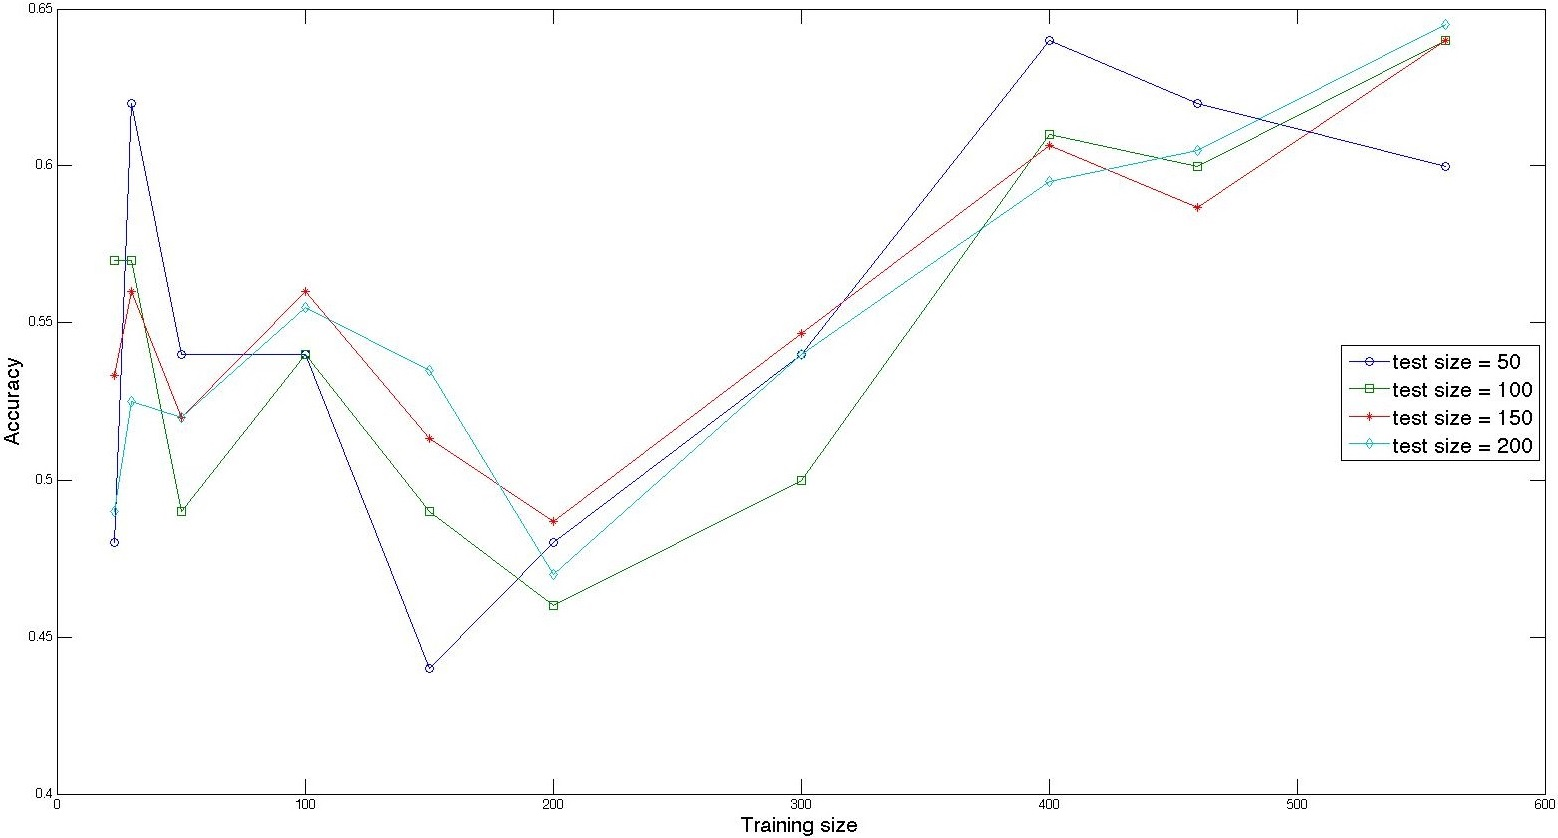
\includegraphics[width=0.5\textwidth]{results/acc.jpg}
	\caption{Accuracy for various test sizes}
\end{figure}
\begin{figure}[H]
	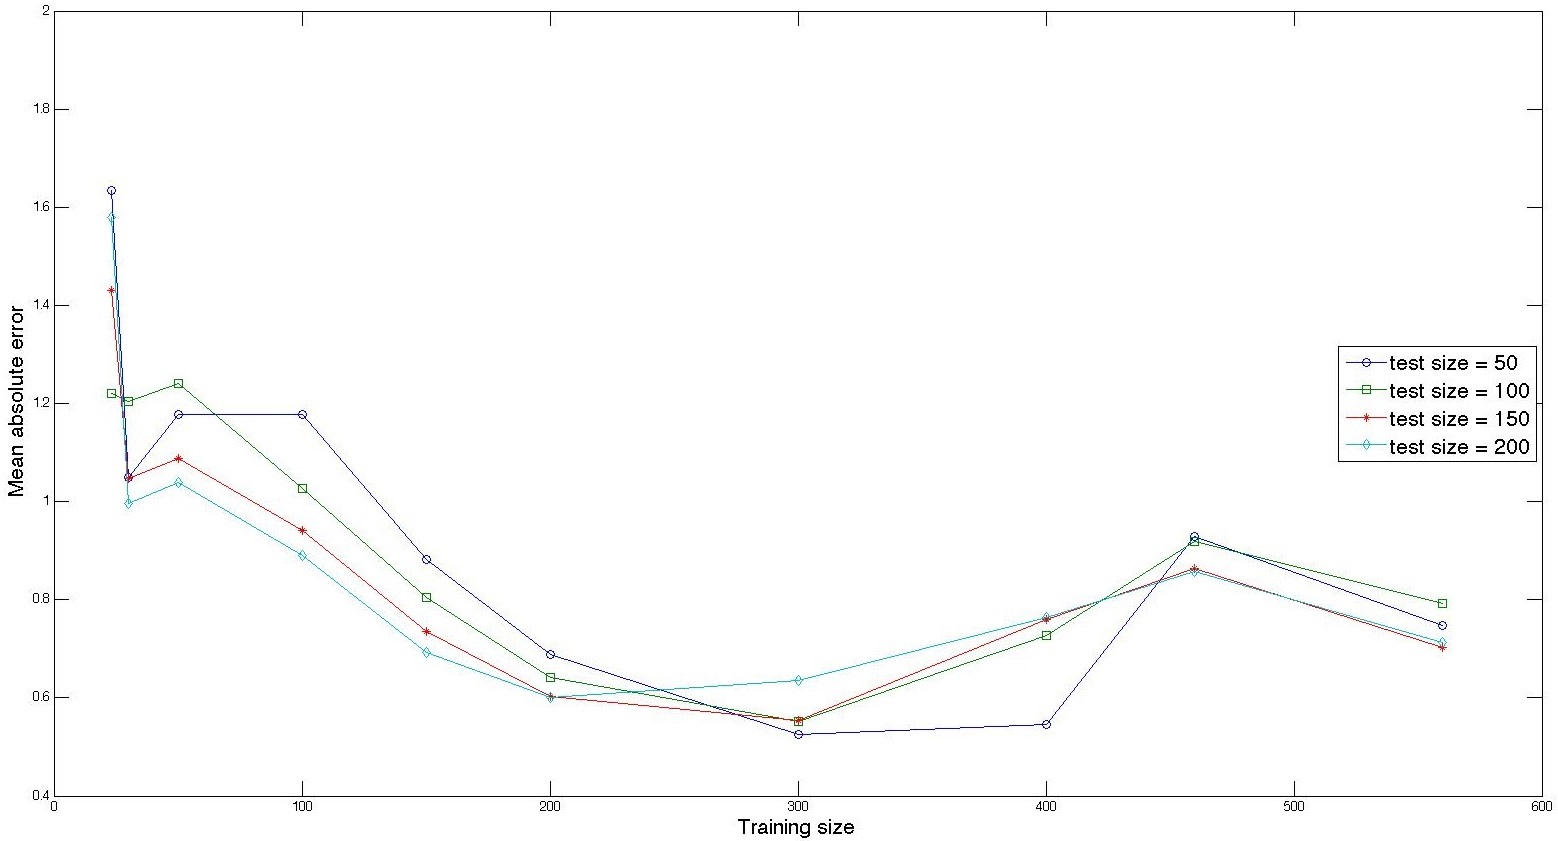
\includegraphics[width=0.5\textwidth]{results/mae.jpg}
	\caption{Mean aboslute error for various test sizes}
\end{figure}
\figurename{6} and \figurename{7} show the accuracy and mean absolute error across test size for a fixed window of last 22-560 training days. When we predict further in the future, our training data becomes less relevant and accuracy decreases, thus we also used a moving window of training set as shown in the two figures below.
\begin{figure}[H]
	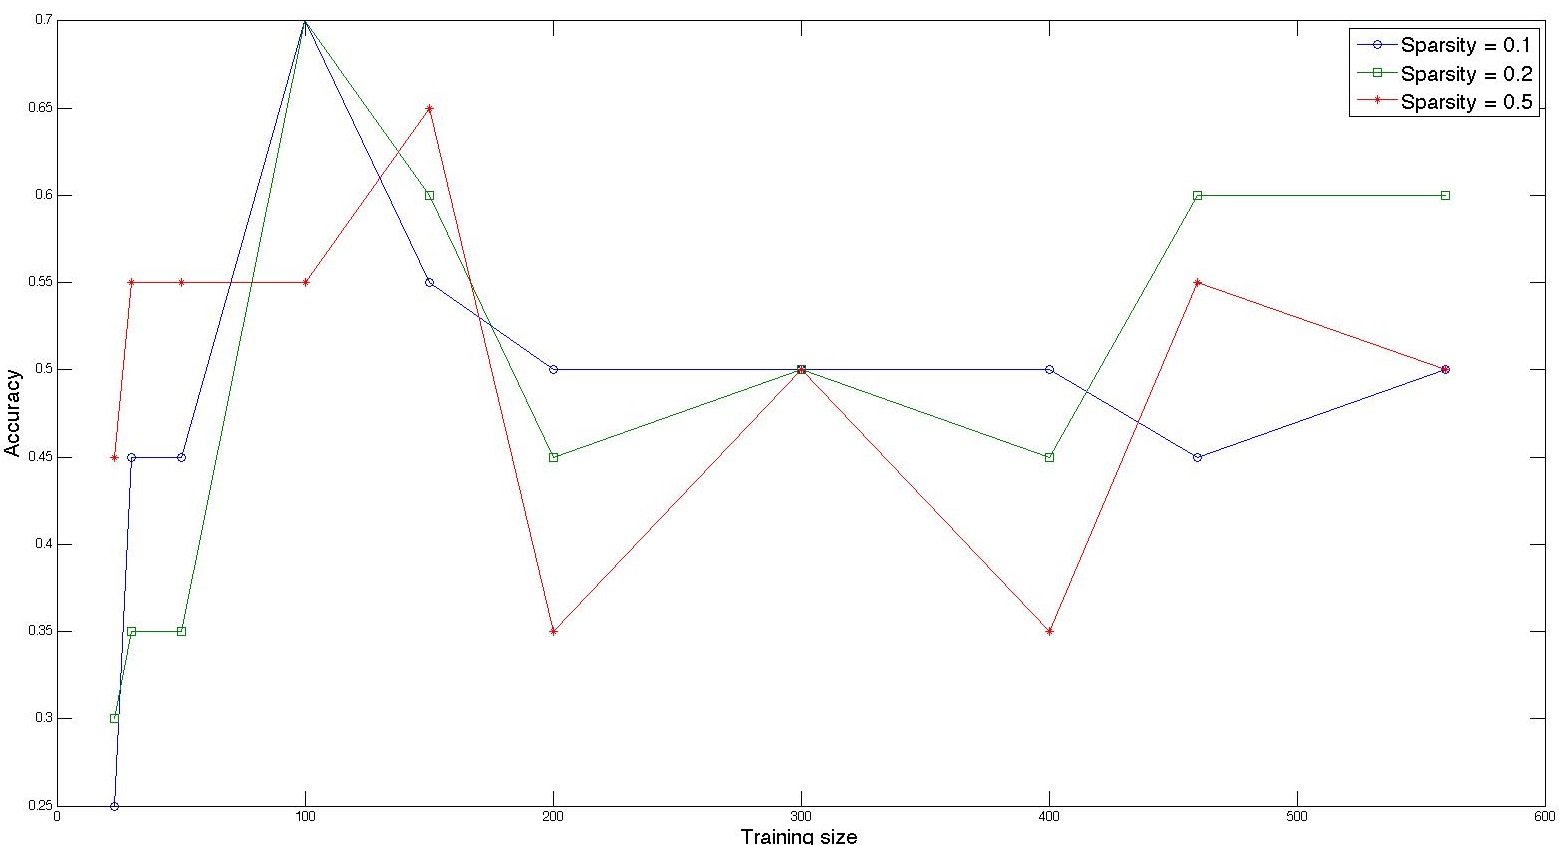
\includegraphics[width=0.5\textwidth]{results/acc2.jpg}
	\caption{Accuracy for various sparsity}
\end{figure}
\begin{figure}[H]
	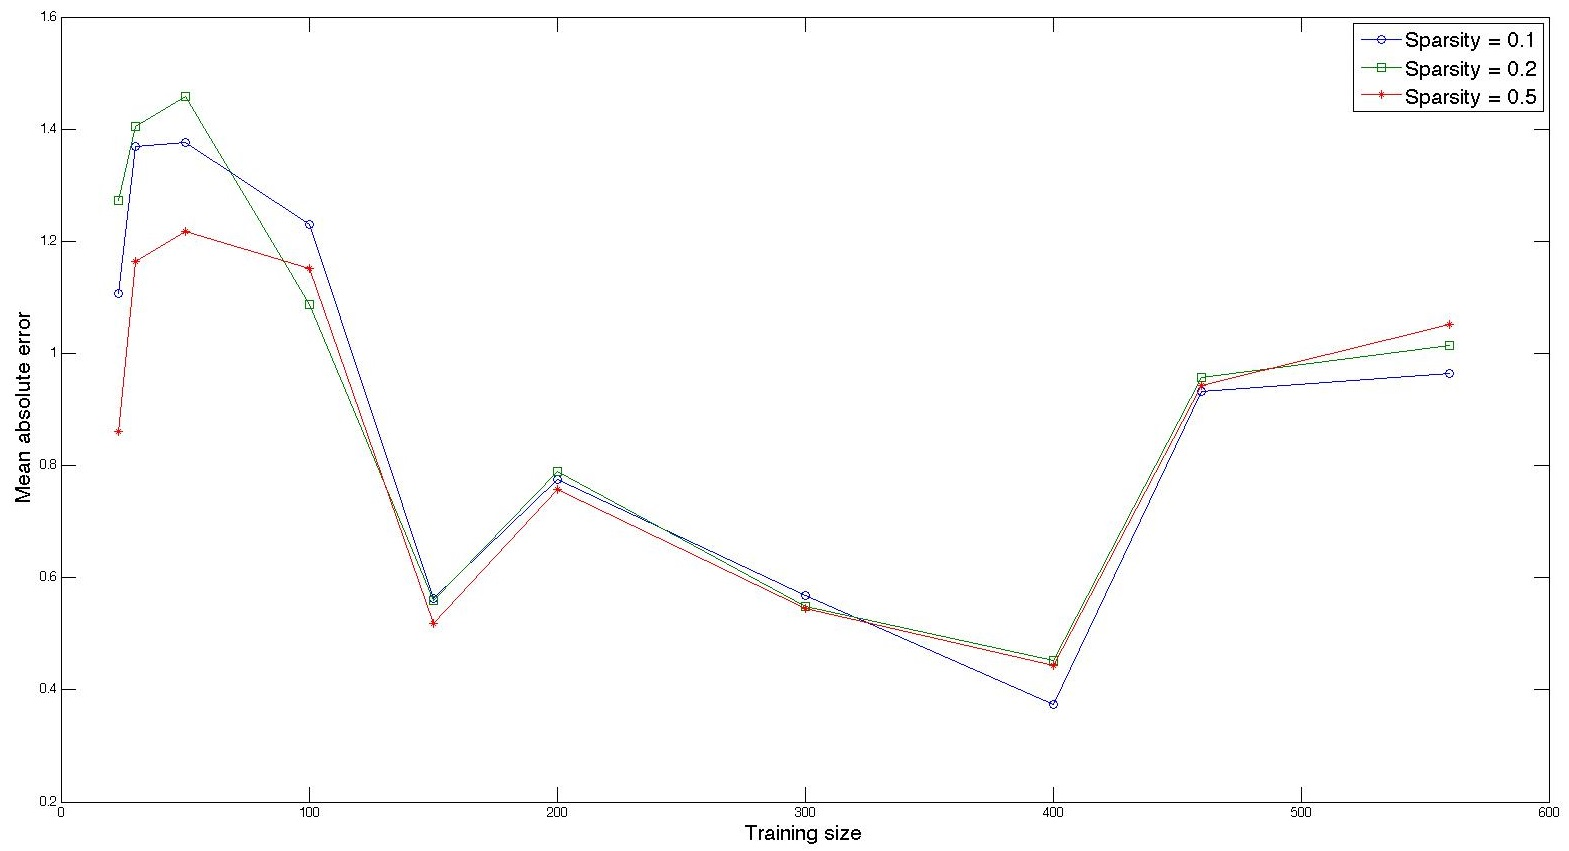
\includegraphics[width=0.5\textwidth]{results/mae2.jpg}
	\caption{Mean abolsute error for various sparsity}
\end{figure}

\figurename{8} and \figurename{9} show the accuracy and mean absolute error across sparsity for a moving window of last 22-560 training days. As recomputing the whole windows is computationally expensive, we only recomputed the coefficients for the training days, but as we can see the best accuracies are approximately similar but we managed to reduce best mean absolute error ot 0.37 from 0.52 in the fixed window.

\begin{figure}[h!]
	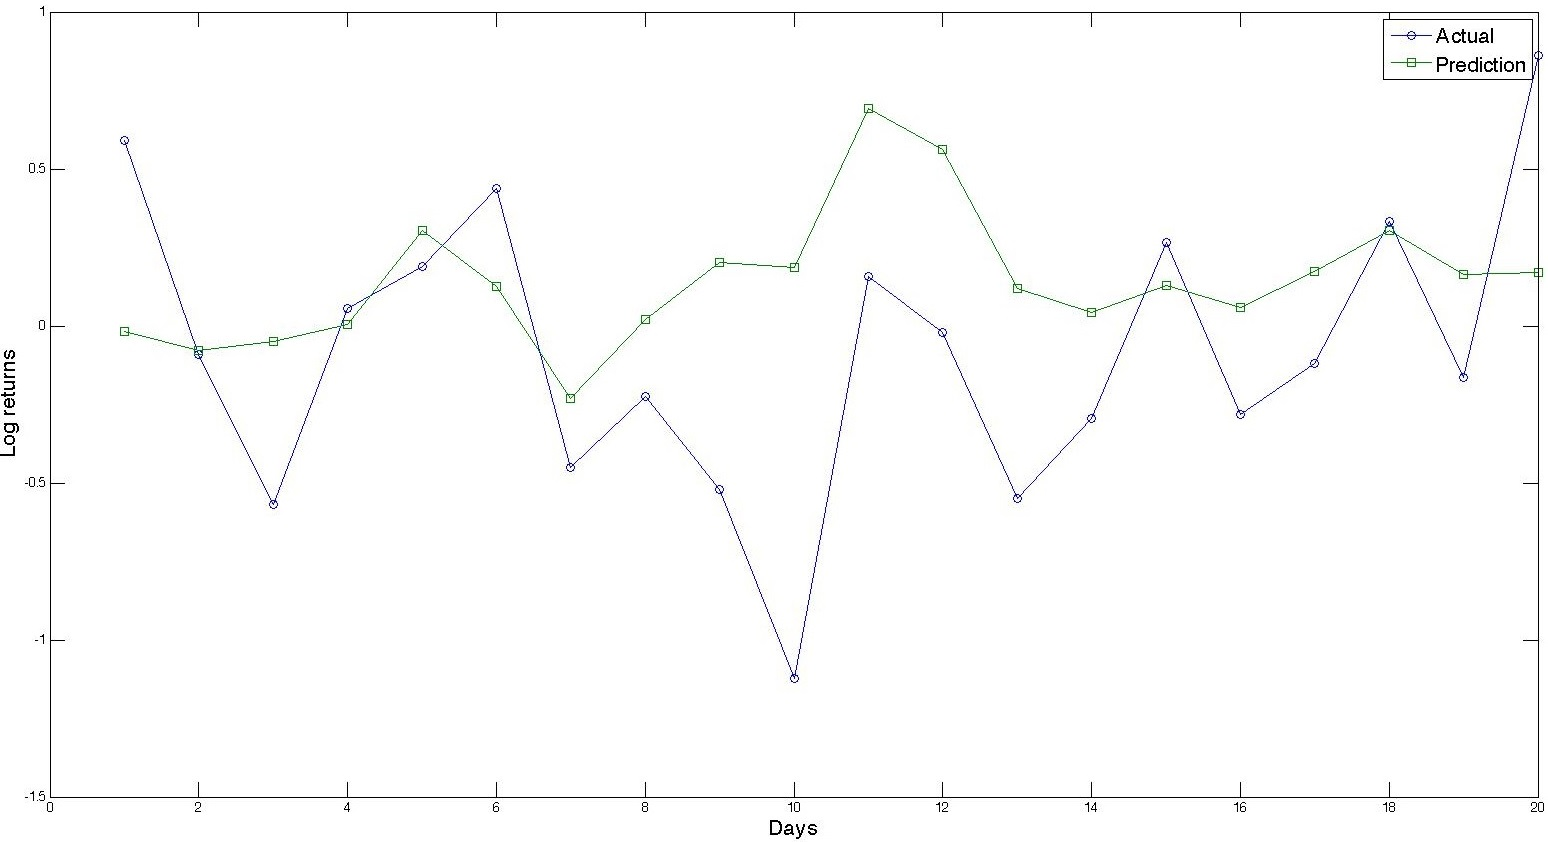
\includegraphics[width=0.5\textwidth]{results/prediction.jpg}
	\caption{Comparison of log returns for sparsity = 0.1, training size = 400}
\end{figure}

\figurename{10} is a log return plot with a moving window of 400 days and sparsity 0.1 having a mean absolute error of 0.37. We can see that qualitatively we can predict the positions of peaks and valleys but not the actual values.





\section{Evaluation}

To evaluate our results in the context of financial predictions, we ran a trading strategy on our test data set, using the predictions of our linear model.

Given a risk-free rate for borrowing leverage, $r$, the Kelly Criterion states that for a security with mean returns $\mu$ and volatility $\sigma$, the optimal fractional investment in the security one should make is $\frac{\mu-r}{\sigma^2}$ \cite{davis2012fractional}. 
todo assumptions
Estimating volatility from the training set and using the predicted next-day returns to calculate the proportion of the commodity tested, silver, to buy, we were able to simulate our performance over the 221-day period:

\begin{figure}[ht]
\vskip 0.2in
\begin{center}
\centerline{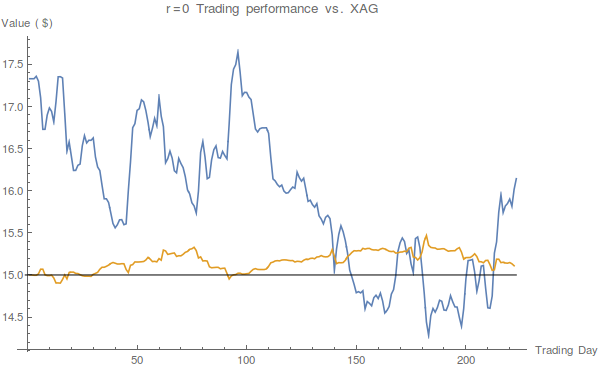
\includegraphics[scale=0.3]{images/sparse-silver.png}}
\caption{Portfolio performance for $r=0$ over time on the test set. Note mistakes (when the net value of our assets, in purple, falls) typically occur from poorly predicting upswings. At the above rate, we make 0.7\% returns on the given investment. We choose an artificial starting investment of \$15 (allowing for partial stock purchases) to keep the scales the same. The black line is the no-risk play.}
\end{center}
\vskip -0.2in
\label{fig:preprocess}
\end{figure}

We don't use the S\&P as a metric for the risk-free rate over this time because it actually fell 1.2\% over the testing period. Using instead a generous estimate of the yearly U.S. Treasury bond yield for the year of the test set, at 0.5\% (but modified to be compounded daily to fit with the per-day trading strategy), we still have some improvement.

The risk free rate did not effect our returns and is only useful as a benchmark to compare our strategy. Over the entire test run, we are only ever confident enough to purchase (or short) an amount of stocks equal to 51.8\% of our current net value, so no leverage is ever used.

Because our model beats all reasonable risk-free rates, there is some (albeit small, financially speaking) predictive power offered by the model. The returns on our net worth fluctuate over the test period with a standard deviation of 0.740\%, and we ended up with 0.727\% gains at the end of the test period.

TODO(Vlad + Ghassen): Add analogous performance summary for model trained without any GDELT information.


\section{Future Work}

\subsection{Improving the Prediction Models}
We have tried different window sizes for both training and testing as well as moving the windows instead of fixing them. We also tried using PCA for LM and ARIMA but found that using Lasso once the orders of AR and MA are determined to be more efficient. Our binary accuracy results are on-par with the state-of-the-art ones. However, it is clear that our prediction, for the simple log return data, is most from the time series lags itself and not GDELT. The sparser our usage of GDELT is, the higher our testing results are. Therefore, we have to either analyze different time series (discussed later in this section) or try to estimate different features of the time series such as extreme values or peaks in the log return. For example, we could work on a logistic regression that classifies days in the top $10\%$ in terms of log return value, as "high", days in the bottom $10\%$ as low and the rest as "medium". In this case, we would be doing two classifiers, one on the "high" and one on the "low" in a similar fashion to exemplar SVM, where we train the high/low with so many negative examples that it has a higher certainty where predicting a peak. Our final result would indicate whether there are peaks (high or low) or if the trading activity is rather normal (medium) or if our results conflict (we get positive for both high and low). Only in the first case where we are sure about one kind of the peaks would we consider the prediction for our trading strategy.

\subsection{Infinite Gaussian Mixture Model}
For clustering news events we have relatively little information for deciding how many clusters there should be. In our $K$-means model, we do a parameter search for values of $K$ from 10 to 5000 on a logarithmic scale. Ideally we would be able to use an infinite Gaussian mixture model that takes in a hyperparameter for a clustering coefficient and automatically determines the number of clusters and therefore remove the need for this imprecise parameter search. 

We attempted using a Dirichlet Process GMM but the implementation we attempted to use was intractable given our computing power. We may attempt to optimize the parameters of the DPGMM in the future or work on limiting the model's training set further. 

\subsection{Filtering GDELT by Commodity}
Up to now, we have been sampling the entire GDELT dataset for news events in order to predict the movement in commodity prices (e.g. silver). Since GDELT contains a large variety of news topics, the majority of the news articles within each day are not related to the specific commodity that we study. A more accurate way to predict the commodity prices would be to implement a filtering pipeline that removes irrelevant news items. This can be achived with natural language processing by selecting news articles that have keywords such as ``silver" and ``commodity". This approach should improve our prediction accuracy because it would remove a significant portion of the noise in GDELT.




\subsection{Software and Data}

All code used is available in an open-source repository.\footnote{\hyperref[https://github.com/vlad17/COS513-Finance]{\texttt{https://github.com/vlad17/COS513-Finance}}} GDELT provides free access to its database as well.\footnote{ \hyperref[http://data.gdeltproject.org/events/index.html]{\texttt{http://data.gdeltproject.org/events/index.html}}}

Commodities pricing data is retrieved using the \texttt{R} package \texttt{quantmod}\footnote{\hyperref[http://www.quantmod.com/]{\texttt{http://www.quantmod.com/}}}, which pulls historical prices using Yahoo.

TODO(Tom): Update our sources for quotes

% Acknowledgements should only appear in the accepted version. 
% \section*{Acknowledgments} 

% In the unusual situation where you want a paper to appear in the
% references without citing it in the main text, use \nocite
% \nocite{langley00}

\bibliography{biblio}
\bibliographystyle{icml2015}


\end{document}
